\begin{itemize}
\item Ahmad Syafrizal Huda (1164062)
\item Annisa Fathoroni (1164067)
\item Puad Hamdani (1164084)
\item Rahmi Roza (1164085)
\item Tasya Wiendhyra (1164086)
\end{itemize}

\section{Definisi RESTful Web Service}
REST merupakan salah satu macam web service yang memasukkan konsep perpindahan antar state. State disini bisa dibayangkan seperti jika browser meminta suatu halaman web, maka server akan mengirimkan state halaman web yang sekarang ke browser. Menurut salah satu perkembangan Tidwell, D., 2001 bernavigasi melalui link-link yang disediakan sama halnya dengan mengganti state dari halaman web. Begitu pula REST bekerja, dengan bernavigasi melalui link-link HTTP untuk melakukan aktivitas tertentu, seakan-akan terjadi perpindahan state satu sama lain \cite{indrawan2017implementasi}.
Pada gambar \ref{labelgambar} menerangkan cara Rest Web Service melakukan request kepada server kemudian server membalasnya dengan result berupa json. Metode tersebut telah dikembangkan oleh Roy Thomas Fielding dalam disertasinya tentang Architectural Style.  Dalam disertasinya tersebut REST (Representational state transfer) didefinisikan sebagai suatu gaya arsitektur perangkat lunak untuk pendistribusian sistem hypermedia seperti WWW \cite{rofiq2017implementasi}.
\begin{figure}[ht]
\centerline{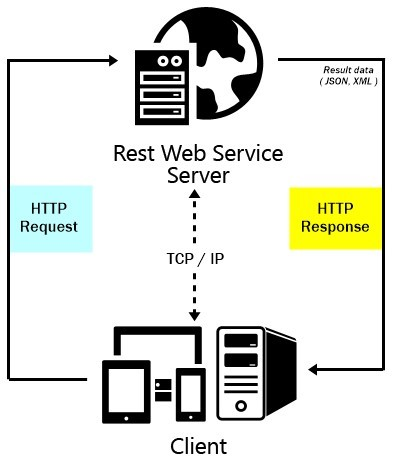
\includegraphics[width=1\textwidth]{figures/1restful.jpg}}
\caption{RESTful}
\label{labelgambar}
\end{figure}

\section{Prinsip atau Karakter Pada RESTful}
RESTful adalah salah satu teknologi web service untuk membuat suatu sistem yang terdistribusi dimana cara kerjanya berdasarkan resource. RESTful sendiri merupakan software yang didesain untuk penekanan pada skalabilitas,kesederhanaan dan kegunaan. Metode dalam REST terdiri dari empat prinsip utama teknologi, yaitu \cite{aji2016penerapan}:
\begin{enumerate}
\item Resource identifier melalui Uniform Resource Identifier (URI), REST Web service mencari sekumpulan sumber daya yang mengidentifikasi interaksi antar klien.
\item Uniform interface, sumber daya yang dimanipulasi CRUD (Create, Read, Update, Delete) menggunakan operasi PUT, GET, POST, dan DELETE.
\item Self-descriptive messages, sumberdaya informasi tidak terikat, sehingga dapat mengakses berbagai format konten (HTML, XML, PDF, JPEG, Plain Text dan lainnya). Metadata pun dapat digunakan.
\item Stateful interactions melalui hyperlinks, setiap interaksi dengan suatu sumber daya bersifat stateless, yaitu request messages tergantung jenis kontennya.
\end{enumerate}

\section{Sejarah RESTful}
REST tidak menarik perhatian banyak ketika pertama kali diperkenalkan pada tahun 2000 oleh Roy Fielding di Universitas California, Irvine, dalam disertasinya akademik, Architectural gaya dan arsitektur perangkat lunak berbasis desain jaringan, yang menganalisa set dari prinsip-prinsip arsitektur perangkat lunak yang menggunakan Web sebagai platform untuk komputasi terdistribusi (Lihat sumber daya untuk link ke disertasi ini). Sekarang, tahun setelah diperkenalkan, utama kerangka untuk REST telah mulai muncul dan masih sedang dikembangkan karena itu dijadwalkan, misalnya, akan menjadi bagian integral dari Java 6 melalui JSR-311 \cite{rodriguez2008restful}.

\section{Contoh-Contoh Penerapan  RESTful}
\subsection{Implementasi RESTful Web Service untuk Sistem Penghitungan Suara Secara Cepat pada Pilkada}
Metode ini yang digunakan oleh penyelenggara pemilihan umum untuk menentukan hasil pilkada. Dengan memanfaatkan teknologi yang ada, proses pengumpulan data hasil perolehan suara bisa dilakukan dengan lebih cepat. Salah satu metode baru yang bisa digunakan untuk melakukan proses tersebut adalah metode perhitungan cepat riil. Metode ini memanfaatkan teknologi informasi dan komunikasi untuk melakukan proses penghitungan suara. Real-quick count mengambil hasil perhitungan dari semua tempat pemungutan suara (TPS). Tetapi hasil tersebut dikirim langsung dari TPS ke lembaga penyedia informasi hasil perhitungan cepat, tidak melalui prosedur seperti pada real count yang mengharuskan pengumpulan data berjenjang, oleh karena itu waktu yang dibutuhkan untuk memperoleh semua hasil suara bisa dioptimalkan. Pada jurnal ini dilakukan perbandingan antara SOAP dan REST pada aplikasi mobile dan multimedia conference. Hasil penelitian yang dilakukan pada aplikasi mobile computing menunjukkan bahwa ukuran pesan pada RESTful web service mencapai 9 sampai 10 kali lebih kecil dibandingkan ukuran pesan dari web service berbasis SOAP \cite{rofiq2017implementasi}.

\subsection{Implementasi RESTful untuk Sales Order dan Sales Tracking Berbasis Mobile}
Bagian penjualan merupakan bagian yang paling penting dalam penjualan produk. Perusahaan membutuhkan sistem yang dapat membantu aktivitas dan pemesanan produk. dengan membuat sebuah Controller terlebih dahulu,yang berperan untuk menentukan informasi apa yang akan disampaikan pada saat client mengakses web service. Dibuat dengan arsitektur REST dengan menggunakan method yang di dukung protokol HTTP seperi method DELETE, UPDATE, CREATE,dll. Aplikasi mobile ini akan menggunakan data dari GPS untuk memastikan lokasi penjual juga dilengkapi barcode untuk mempercepat input data barang \cite{kurniawan2015implementasi}.

\subsection{Implementasi REST Web Service Pada Aplikasi Pengolah Pesan Yahoo Messenger Pada CV. Meliana Pratama}
Mengimplementasikan REST Web Service pada aplikasi pengolah pesan Yahoo Messenger (YM). Aplikasi REST Web Service dapat dijadikan sebagai miidleware antara aplikasi pengolahan pesan Yahoo Messenger (YM) dengan database, sehingga proses transaksi ke database menjadil lebih efisien. Hal ini dikarenakan aplikasi client tidak perlu mengetahui database apa yang digunakan oleh server \cite{ikrom2015implementasi}.

\subsection{Implementasi RESTful Web Service Pada Aplikasi Iklan Baris Online}
Pada implementasi aplikasi ini menerapkan restful web service yang dimana server akan berinteraksi dengan client pada interface yang sama atau seragam. Server akan meng-host resource sedangakn client akan menjadi konsumen dari resource yang disediakan server. Pada saat server meminta atau request data script request akan dikirim dari client ke server berbentuk alamat url yang kemudian memanggil file PHP yang mengakses data dari databse server. saat pengambilan data, client akan memanfaatkan API yang terdapat dalam server. Setelah mendapat data dari client, server kemudian akan menyebar informasi yang dibutuhkan berupa kebutuhan barang/jasa yang bersangkutan kepada member atau client \cite{fauziah2014aplikasi}.

\subsection{Implementasi Protokol OAuth 1.0 Sebagai Autentikasi pada Aplikasi SMS Blast Berbasis Android}
Sebuah aplikasi SMS Blast berbasis Android dan sebuah web service yang digunakan oleh aplikasi untuk melakukan request terhadap data nomor telepon terhadap data yang sudah ada. OAuth menggunakan token pada setiap request. Web service akan membangkitkan token yang berbeda pada setiap request dari consumer. Penggunaan token ini dapat meminimalkan kemungkinan terjadinya serangan Man in the Middle Attack dan Hijacking Attack
\cite{saputra2017implementasi}

\subsection{Implementasi RESTful Web Service One Chip Multi-Client Untuk Mengoptimalkan Penjualan Pulsa All Operator}
One  Chip  All  Operator adalah sebuah chip untuk pengisian pulsa kesemua operator selluler GSM dan CDMA bahkan juga dapat digunakan untuk pengisian pulsa listrik atau listrik prabayar. Chip atau kartu perdana  yang  digunakan bukan kartu Khusus atau tidak harus dipesan kedealer penyedia pelayanan pengisian pulsa,Chip yang   digunakan cukup perdana biasa,jadi nomor  yang dipakai sehari-hari dapat dijadikan sebagai chip untuk pengIsian pulsa ke semua operator. Proses awal yang dilakuakanya itu peses deployment restful  web  service. Deployment  restful web service  merupakan proses menjalankan web service pada server seperti apache tomcat agar aplikasi client dapat mengakses service database\cite{indrawan2017implementasi}.

\subsection{Implementasi Protocol Buffers pada Aplikasi Weblog Client dan Server}
Web service yang digunakan untuk mengirimkan dan menerima   protobuf  messages adalah  RESTful  web service  yang  merupakan  teknologi  web  service  yang ringan dan mudah diimplementasikan. Client mengirimkan data yang telah diserialisasikan dalam bentuk protobuf message melalui  HTTP  request kepada RESTful  service pada server. Protobuf  message kemudian diubah menjadi data semula dengan program deserialisasi yang telah ada di server \cite{wibowo2011implementasi}.

\subsection{Implementasi Restful Web Service Menggunakan AsyncTask pada Aplikasi Library Automation Berbasis Android}
Dengan menggunakan aplikasi Library automation berbasis android ini diharapkan dapat mempermudah untuk mengakses informasi terkait referensi yang terdapat pada perpustakaan fisik penggunaan RESTful web service dengam menggunakan AsyncTask sebagai prosesnya juga dinilai cukup baik dari segi penggunaan. Diharapkan untuk pengembangan selanjutnya meningkatkan akurasi pencarian supaya end user tidak merasa bingung saat mencari informasi \cite{yudhistiraimplementasi}.

\subsection{Penerepan Restful pada Aplikasi Ayo Piknik Indonesis Berbasis Android}
Aplikasi Ayo Piknik Indonesia berbasis android yang berbasis dengan Web-server menggunakan metode Restful Webservice yang bisa menampilkan informasi wisata dengan cepat dan tepat serta pengguna juga dapat memberikan usulan tempat wisata yang baru. Kemudian akan dilakukan verifikasi agar bisa ditampilkan. Selain itu aplikasi ini juga  dapat menambahkan data wisata dengan google maps untuk memudahkan wisatawan ataupun penduduk lokal \cite{aji2016penerapan}.

\subsection{Implementasi PHP Web Service Sebagai Penyedia Data Aplikasi Mobile}
Dapat disimpulkan bahwa PHP Web Service bisa diimplementasikan dalam aplikasi mobile yang membutuhkan data dinamis. Pengujian atas web service bisa dilakukan dengan membuat file PHP secara manual ataupun menggunakan SOAP web service. Untuk memudahkan pemanggilan data bisa dilakukan modifikasi dengan memberikan layer tambahan berupa PHP File yang memanggil pada SOAP web service \cite{surendra2014implementasi}.

\subsection{RESTful Web Service Untuk Sistem Pencatatan Transaksi Studi Kasus PT.XYZ}
PT.XYZ merupakan sebuah PT yang bergerak dalam bidang pemasaran perhiasan yang terletak di daerah Semarang.Dalam kesehariannya,terdapat transaksi-transaksi yang mempengaruhi jumlah stok barang, pencatatan dan laporan transaksi yang dilakukan. Proses tersbut berdampak pada penyesuaian data antara data pergudangan dan data pencatatan transaksi,dikarenakan terdapat beberapa database yang digunakan secara terpisah dan aplikasi-aplikasi yang berbeda.
Pemanfaatan Web Service RESTful pada sistem transaksi PT.XYZ memfokuskan pada integrasi setiap sistem yang berbeda. Request sumberdaya yang dilakukan client memanfaatkan URL yang datanya akan disertakan di HTTP header dan kemudian dikirimkan ke web service menggunakan tipe konten application/x-www-form-URLencoded untuk melakukan validasi pada middleware RESTful. dan setiap respon elalu menggunakan format standar yaitu JSON \cite{tanaem2016restful}.

\subsection{MONITORING ABSENSI HARIAN KEPEGAWAIAN PADA INSTANSI PEMERINTAHAN KOTA MAKASSAR BERBASIS RESTFUL API}
Adanya monitoring absensi kepegawaian pada instansi pemerintah kota makassar menggunakan RESTful Api maka dapat menjembatani beragamnya perangkat akses informasi dengan sistemnya masing-masing dalam hal mengakses data absensi kepegawaian dan lebih terkontrol, serta dengan pemanfaatan teknologi RESTful Api maka dapat lebih mengoptimalkan perangkat akses informasi dari yang membutuhkan sehingga membuat pengaksesan infomasi absensi dapat menjadi lebih mudah dan praktis \cite{sy2017monitoring}.

\section{Metode Pengembangan RESTful Pada Web Service}
\subsection{Pengembangan Sistem Informasi RESTful Web Service}
Pengembangan sistem informasi kependudukan berbasis mobile dan restful pada web service yaitu\cite{kurniawati2016pengembangan}:
\begin{enumerate}
\item REST Web Service pada tahap ini akan dibuat web service yang diletakkan pada server pusat untuk mengolah data JSON. Web service memiliki 3 method yaitu json decode yaitu untuk parsing data masukan, StoreData dan json encode parsing untuk data keluaran. Parameter masukan dari database SQLite ke MySQL tampak pada gambar 5, akan diparsing ke dalam format Array. StoreData yang berhubungan langsung dengan database dalam proses input, status gagal atau sukses akan disimpan dalam Array dan diolah lagi menjadi format JSON sebagai keluaran dari web service.
\item Aplikasi Android Antarmuka aplikasi android saat dijalankan akan muncul form login. Pengguna aplikasi yaitu kepala lingkungan memasukkan username dan password kemudian tekan tombol login
\end{enumerate}

\subsection{Pengembangan Sistem Informasi Kependudukan Berbasis Moblie Dan RESTFful Web Service}
Sensus biasa dilakukan secara manual, yaitu door-to-door ke setiap rumah warga namun hal tersebut membutuhkan waktu yang lama dan tidak cukup efektif, lalu dibuat solusi dari permasalahan tersebut dengan mengintegrasikan RESTful web service pada perangkat Android. Diimplementasikan pada Android karena Android memiliki kelebihan dapat mengakses database secara offline yaitu SQLite sehingga lokasi yang berada di pedalaman tetap dapat terinputkan ke database meski tidak ada jaringan internet.
Cara kerjanya yaitu petugas sensus akan memasukan data di perangkat android, yang kemudian datanya akan dimasukkan kedalam database. Webservice RESTful ini berfungsi sebagai komunikator antara android dengan database pusat. Web service ini diletakkan di server pusat untuk mengolah data JSON. Parameter masukkan dari SQLite ke MySQL akan di parsing ke format array yang diubah lagi menjadi JSON sebagai hasil dari web servicenya \cite{kurniawati2016pengembangan}.

\section{Kelebihan dan Kekurangan RESTful Web Service}
Pada tabel \ref{table:contoh} merupakan kelebihan dan kekurangan daripada RESTful Web Service dimana RESTful Web Service ini sangat berguna dalam implementasinya \cite{nugroho2012perbandingan}.
\begin{table}[h]
\begin{tabular}{|c|c|c|}
\hline
Jenis Web Service&Kelebihan&Kekurangan\\
\hline
RESTful Webs Service&-Implementasi RESTful Web Service relatif& -Struktur data yang sangat kompleks\\
&sederhana dalam hal pemrogramannya karena& sukar diadaptasi ke dalam URL.\\
&menggunakan standar-standar yang telah&\\
&diterima secara luas (HTTP, XML, dan URL).&\\
&-Server dan klien HTTP dikenali&-Implementasi dan kinerjanya sangat bergantung\\
&oleh sebagian besar bahasa pemrograman&pada kapasitas jaringan yang digunakan\\
&dan hampir semua platform perangkat&\\
&keras/perangkat lunak yang saat ini populer.&\\
\hline
\end{tabular}
\label{table:contoh}
\end{table}

\section{Kesimpulan}
REST adalah tidak selalu pilihan yang tepat. Itu telah tertangkap sebagai cara untuk desain Web services dengan kurang ketergantungan pada berpemilik middleware (misalnya, aplikasi server) daripada jenis SOAP dan WSDL berbasis. Dan dalam arti, REST adalah kembali ke Web cara itu sebelum usia server aplikasi besar, melalui penekanan pada awal Internet standar, URI dan HTTP. Seperti yang Anda telah dikaji dalam prinsip-prinsip yang disebut RESTful interface Design, XML di atas HTTP adalah antarmuka yang kuat yang memungkinkan aplikasi internal, seperti Asynchronous JavaScript + XML (Ajax)-berbasis antarmuka pengguna kustom, untuk dengan mudah menghubungkan, alamat, dan mengkonsumsi sumber daya. Pada kenyataannya, sangat sesuai antara Ajax dan REST telah meningkat jumlah perhatian REST semakin hari ini \cite{rodriguez2008restful}.

\section{IMPLEMENTASI RESTFUL WEB SERVICE ONE CHIP MULTI-CLIENT UNTUK MENGOPTIMALKAN PENJUALAN PULSA ALL OPERATOR}
Jenis web service yang digunakan pada sistem ini adalah Restful Web Service. Web service jenis ini dapat membantu mengatasi permasalahan yang ada pada Wincell karena REST digunakan sebagai prinsip dasar untuk transfer data secara stateless pada data yang dapat di akses menggunakan protokol HTTP dan REST dapat di representasikan dalam berbagai format, antara lain teks, XML, JSON, dan lain-lain
\cite{indrawan2017implementasi}.

\section{Implementasi Pull Message dengan Menggunakan RESTful Web Service pada Komunikasi Wireless Sensor}
Wireless Sensor Network merupakan jaringan yang menggunakan dan memiliki jumlah sensor node yang sangat banyak. untuk meringankan biaya sensor node biasanya diterapkan menggunakan Arduino. Mekanisme pull message dengan menggunakan Restful Web Service dapat diimplementasikan pada proses komunikasi di dalam WSN. Sensor node (Arduino) dapat digunakan sebagai web server dan bisa menangani request dari banyak client melalui pemanfaatan thread sederhana, sedangkan sink node (Raspberry Pi) dapat melakukan proses pull message dengan menggunakan protokol Restful Web Service pada komunikasi WSN. 
\cite{hidayatullah2017implementasi}
